\documentclass[../main.tex]{subfiles}

\begin{document}
\chapter{Physically Based Rendering}

\section{Wstęp}

W początkach lat 2000 najpopularniejszym modelem wykorzystywanym w grach był
model Blinna-Phonga, który nie wymagał dużej mocy obliczeniowej do oświetlenia
nawet złożonych scen. Model ten możemy opisać prostym równaniem:

\[
	I(p) = k_a I_a +
		\sum_{m \in L} \left( {
			k_d \max\left({ L_m \cdot H, 0 }\right) +
			k_s (R_m \cdot V)^{\alpha} i_{m,s}
	} \right)
\]

gdzie $ H = \frac{V+L}{||V+L||} $.

Jak widać model bierze pod uwagę poniższe stałe opisujące materiał:

\begin{itemize}
\item $k_a$ - współczynnik odbicia światła otoczenia
\item $k_d$ - współczynnik odbicia światła rozproszonego
\item $k_s$ - współczynnik odbicia światła lustrzanego
\end{itemize}

Jak widać, powyższe stałe są tak naprawde kolorami różnych typów interakcji
wiązki światła z powierzchnią. Kolor odbicia zależy w bardzo dużym stopniu od
artysty i jego wyobrażenia o zachowaniu światła w danym środowisku, nie wynika
on jasno z właściwości materiału, lecz zwykłego domysłu jak poszukiwany
materiał się zachowa i w jaki sposób będzie połyskiwał. Doprowadza to sytuacji,
w których obiekt, dla którego stworzone są tekstury może wyglądać bardzo dobrze
w jednym otoczeniu, by w drugim wyglądać nienaturalnie: zaprojektowany model
wraz z mapami może bardzo dobrze prezentować się na zewnątrz pośród trawy, lecz
w słabo oświetlonej jaskini nie będzie sprawiał wrażenia naturalnego, wrażenia
istnienia w i razem z tym miejscem. Zatem jednym z głównych problemów prostych
modeli oświetlenia jest to, że bardzo często nie wyglądają one naturalnie w
różnych warunkach oświetlenia.

Podejście PBR wychodzi naprzeciw oczekiwaniom i rozwiązuje ten problem tworząc
podejścia tworzenia sceny w którym operujemy na faktycznym opisie materii, nie
na domysłach i zmyśle artystycznym, przekładając odpowiedzialność za poprawny
wygląd w dowolnej scenie na modele matematyczne.

Kolejnym problemem prostych modeli oświetlenia jest brak zachowania
podstawowych zasad fizycznych, w tym zasady zachowania energii. Ze względu na
prostą strukturę równania Blinna-Phonga, nie jest możliwa kontrola jaka część
energii zostaje rozproszona, a jaka odbita. Bez ingerencji artysty (lub
programisty) często dochodzi do sytuacji w której refleksy są prześwietlone w
wyniku "wygenerowania" energii przez obszar powierzchni - w miejscu w którym
więcej światła ulega odbiciu, mniej światła może może ulec rozproszeniu. Model
nie bierze tego zjawiska pod uwagę przez co powstają nienaturalne refleksy.

Model Blinna-Phonga również nie jest w stanie obsłużyć wielu materiałów,
w tym metali, które cechują się pełną absorpcją światła załamanego.

\section{Analiza geometryczna wiązki światła}

Rozważania na temat modelu zgodnego z fizyką rozpoczniemy od zrozumienia natury
wiązki światła. Sposób w jaki wiązka światła zachowuje się po zderzeniu z
idealnie równą powierzchnią jest fundamentem całej dziedziny metod poprawnych
fizycznie.

Wiązka światła uderzająca w powierzchnię rozdziela się na dwie części, poprzez
dwa zjawiska: odbicie oraz refrakcję.

Część energii wiązki światła odbija się, jest ona wysłana na zewnątrz obiektu
bez wchodzenia w jego materię.

Część energii, która została uległa refrakcji wchodzi wgłąb obiektu, gdzie
zachodzą kolejne kolizje z atomami materii, przez co znów dochodzi do
powyższego zjawiska, tym razem we wnętrzu obiektu. Część tego światła może
wydostać się z obiektu i dotrzeć do obserwatora, pozostała część zostanie
pochłonięta i zamieniona na inne rodzaje energii np. ciepło. Zauważmy, że
energia która dociera do obserwatora musi być mniejsza lub równa energii wiązki
światła - ta właściwość jest jednym z filarów podejścia fizycznie poprawnego.

W modelach matematycznych wymienionych w tej pracy zakładamy, że ponowne
wyjście energii która była poddana refrakcji następuje w tym samym punkcie, w
którym promień zderzył się z powierzchnią (rys.
\ref{fig:ReflectionRefraction}). Istnieją techniki które biorą pod uwagę
możliwość ucieczki energii w innym miejscu, ale skomplikowałyby one rozważania
na których skupia się ta praca.  (Subsurface scattering, renderowanie skóry
itd.)

\begin{figure}[ht]
  \centering
  \begin{tikzpicture}
    %\draw[help lines] (-5,-1) grid (5,5);

		\coordinate (left) at (-3,0);
		\coordinate (right) at (3,0);
    \draw [ultra thick] (left) -- (right);

		\coordinate (normal) at (0,3);
		\coordinate (invnormal) at (0,-3);

    \draw  [-{Triangle[scale=2]}] (invnormal) -- (normal) node [above] {$N$};

		\coordinate (orig) at (0,0);
		\coordinate (light) at (45:3);
		\coordinate (reflection) at (135:3);
		\coordinate (refraction) at (205:3);

    \draw  [-{Triangle[scale=2]}] (orig) -- (reflection)
      node [midway, above] {$r$};
    \draw  [-{Triangle[scale=2]}] (orig) -- (refraction)
      node [midway, above] {$t$};
    \draw  [-{Triangle[scale=2]}] (light) -- (orig);

    \draw pic[draw=black, <->, "$\alpha_i$", angle eccentricity=1.5]
			{angle = light--orig--normal};

    \draw pic[draw=black, <->, "$\alpha_r$", angle eccentricity=1.5]
			{angle = normal--orig--reflection};

    \draw pic[draw=black, <->, "$\beta$", angle eccentricity=1.5]
			{angle = refraction--orig--invnormal};


    \node at (2.8,+0.25) {$n_1$};
    \node at (2.8,-0.25) {$n_2$};

    \draw [fill] (light) circle [radius=0.05] node [above] {\Large\faLightbulbO};

  \end{tikzpicture}
  \caption{Przybliżony model interakcji wiązki światła z powierzchnią}
\end{figure}

\textbf{Prawo odbicia} mówi, że kąty padania wiązki światła $\theta_i$ i jej
odbicia $\theta_r$ od płaszczyznę są równe ($\theta_i = \theta_r$);

\textbf{Prawo Snella} opisuje zmianę kierunku promienia światła przy przejściu
przez granicę dwoma jednorodnymi ośrodkami o współczynnikach załamania $n_i$
poniższym równaniem:

\begin{displaymath}
  \frac{\sin\alpha}{\sin\beta} =
    \frac{n_2}{n_1} = n_{21}
\end{displaymath}

\textbf{Równania Fresnela} (ang. \textit{Fresnel equations}) opisują stosunek
energii światła odbitego do światła załamanego, równania Fresnela również
opisują przesunięcie fazowe fali światła, ale nie będziemy tego brali pod
uwagę.

% Rysunek odbicia z płaską powierzchnią (model uproszczony)
\begin{figure}[h]
  \centering
  \begin{tikzpicture}
    %\draw[help lines] (-5,-1) grid (5,5);
    \draw [thick] (-5.0,0.0) -- (5.0,0.0);

    % Specular
    \foreach \i in {0,...,5} {
      \pgfmathtruncatemacro{\angle}{90+30+(\i / 5) * 30};
      \draw [-Triangle, blue] (0,0) -- ( {3*cos(\angle)}, {3*sin(\angle)} );
    }

    % Diffuse
    \foreach \i in {1,...,15} {
      \pgfmathtruncatemacro{\angle}{(\i / 16) * 180};
      \draw [-Triangle, gray] (0,0) -- ( {2*cos(\angle)}, {2*sin(\angle)} );
    }

    \draw [fill] (2,2) circle [radius=0.05] node [above] {\Large\faLightbulbO};
    \draw [-{Triangle[scale=2]}] (2,2) -- (0,0);
  \end{tikzpicture}
  \caption{Przybliżony model interakcji wiązki światła z powierzchnią}
  \label{fig:ReflectionRefraction}
\end{figure}

W naturze żaden materiał jest idealnym lustrem, w odpowiednio dużym
przybliżeniu zauważymy nierówności niedostrzegalne gołym okiem, a w odniesieniu
do grafiki komputerowej nierówności są dużo mniejsze od pojedynczego piksela
(rys. \ref{fig:Microstructure}).

\begin{figure}[h]
  \centering
  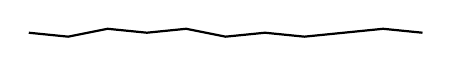
\begin{tikzpicture}
    \draw [thick]
      (0.0,0.15) --
      (0.5,0.10) --
      (1.0,0.20) --
      (1.5,0.15) --
      (2.0,0.20) --
      (2.5,0.10) --
      (3.0,0.15) --
      (3.5,0.10) --
      (4.0,0.15) --
      (4.5,0.20) --
      (5.0,0.15);
  \end{tikzpicture}
  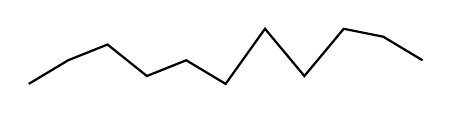
\begin{tikzpicture}
    \draw [thick]
      (0.0,0.1) --
      (0.5,0.4) --
      (1.0,0.6) --
      (1.5,0.2) --
      (2.0,0.4) --
      (2.5,0.1) --
      (3.0,0.8) --
      (3.5,0.2) --
      (4.0,0.8) --
      (4.5,0.7) --
      (5.0,0.4);
  \end{tikzpicture}
  \vspace{0.25cm}
  \caption{Mikrostruktura powierzchni o różnej chropowatości}
	\label{fig:Microstructure}
\end{figure}

Zdefiniujmy teraz kilka funkcji, które pomogą nam w wymodelowaniu powyższych
zjawisk.

Funkcja rozkładu normalnych (ang. \textit{Normal Distribution Function, NDF})
opisuje rozkład normalnych mikropowierzchni na pewnej powierzchni o
współczynniku $\alpha$. Każda funkcja rozkładu normalnych w postaci
znormalizowanej spełnia warunek \cite{NDFReed}:

\[
  \int_{\omega} {
    D(\omega_i)
    (n \cdot \omega_i)
    d \omega_i
  } = 1
\]

Przyciemnienie geometryczne (ang. \textit{Geometric Shadowing}) odpowiada za
zjawiska rzucania cieni w obrębie mikropowierzchni, w związku z czym światło
które pada pod pewnym kątem nie odbija się od całości powierzchni (ang.
\textit{shadowing}, rys. \ref{fig:GeometricShadowing}) oraz zasłaniania
promieni odbitych od powierzchni zmierzających do obserwatora przez inne
elementy tej powierzchni w związku z czym światło odbite nie dociera w całości
do obserwatora. W realnym świecie promień po takim zderzeniu nie znika, ale
uproszczone modele traktują takie zachowanie jako absorpcję światła przez
powierzchnię.

\begin{figure}[h]
  \centering
  \begin{tikzpicture}
    \draw [thick, name path=surface]
      (-2.5,0.8) -- (-2.0,0.4) -- (-1.5,0.7) -- (-1.0,0.2) -- (-0.5,0.5) --
      (0.0,0.1) --
      (0.5,0.8) -- (1.0,0.2) -- (1.5,0.8) -- (2.0,0.7) -- (2.5,0.3);

		\foreach \i in {-3.00,-2.50,...,1.5} {
			\coordinate (rayOrigin) at ($ (\i,0)+(40:3) $);
			\coordinate (rayTarget) at (\i,0);

			\path [name path=ray] (rayOrigin)--(rayTarget);
			\draw [name intersections={of=surface and ray, by=x, sort by=ray}];

			\draw [dotted, thick, orange] (rayOrigin)--(rayTarget);
			\draw [very thick, orange] (rayOrigin)--(x);
		}

    \draw [thick, name path=surface]
      (-2.5,0.8) -- (-2.0,0.4) -- (-1.5,0.7) -- (-1.0,0.2) -- (-0.5,0.5) --
      (0.0,0.1) --
      (0.5,0.8) -- (1.0,0.2) -- (1.5,0.8) -- (2.0,0.7) -- (2.5,0.3);

  \end{tikzpicture}
  \vspace{0.25cm}
  \caption{Samozacienianie wewnątrz mikropowierzchni}
	\label{fig:GeometricShadowing}
\end{figure}

Współczynnik Fresnela opisuje stosunek światła odbitego do światła załamanego
na danej powierzchni pod danym kątem. Popularnymi modelami opisującymi tą
relację są:

\begin{itemize}
\item aproksymacja Schlicka: $F = F_0 + (1 - F_0)(1-V \cdot H)^5$
\item aproksymacja \textit{Spherical Gaussian} \cite{SphericalGaussianLegarde}:
	$ F = F_0 +(1−F_0) 2^{
		\left(−5.55473\left(V \cdot H\right)−6.98316\right) (V \cdot H)
	} $
\end{itemize}

\begin{figure}[ht]
	\centering
  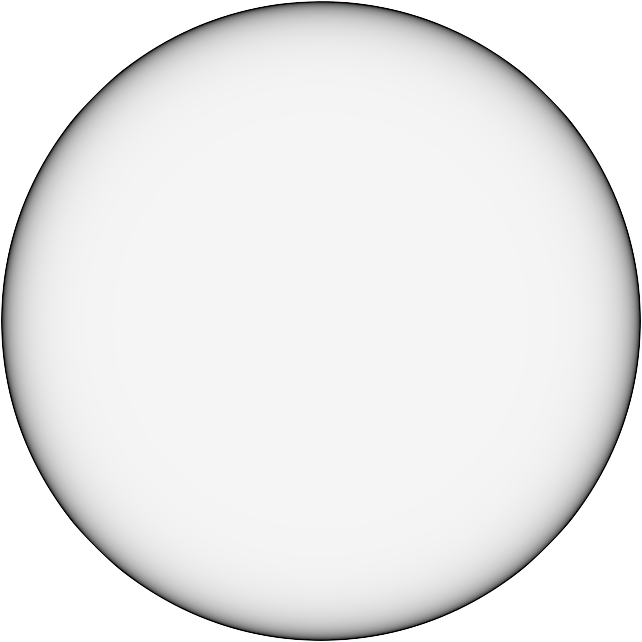
\includegraphics[width=3cm]{pbr/fresnel}
	\caption{Odwrócony współczynnik Fresnela, aproksymacja Schlicka}
\end{figure}

Modele GTR (General Trowbridge-Reitz) i inne bazują na podejściu
mikropowierzchni z których każda zachowuje się jak powierzchnia idealna. Modele
te, szacują statystycznie jaka część promieni przybywająca z kierunku $w_i$
zostanie odbita w zadanym kierunku $w_o$. Funkcję tą, którą dalej będziemy
nazywać funkcją *BRDF* (ang. *bidirectional reflectance distribution
function*).

Całość odbitego światła w kierunku $w_o$ oznaczymy przez:

$$
L_0 = \int_{\Omega} {
    f_r(p, \omega_i, \omega_o)
    L_i(w_i)
    (n \cdot \omega_i)
    d \omega_i
}
$$

Powyższe równanie nazywamy równaniem renderingu (ang. *render equatiton*).

\section{Podstawowe pojęcia radiometryczne}

Rozpocznijmy od podstawowego budulca wiązki światła - fotonu. Energia fotonu
o długości fali $\lambda$ może zostać policzona ze wzoru

$$ Q = \frac{hc}{\lambda} $$

gdzie $h$ jest stałą Plancka a $c$ prędkością światła.

Strumień promieniowania (inaczej moc promieniowania, ang. *radiant flux*) to
całkowita ilość energii przechodząca przez określoną powierzchnię w czasie
jednostkowym. Powyższe pojęcie dotyczy wszystkich fal elektromagmetycznych,
zatem jest ono poprawne również dla światła. Jednostką strumienia
promieniowania jest Watt ($\text{W}$).

$$
\Phi = \lim_{\Delta t \rightarrow 0}{
    \frac{\Delta Q}{\Delta t}=\frac{dQ}{dt}
}
$$

Irradiancją nazywamy strumień promieniowania na jednostkę powierzchni.

$$
E(p) =
    \lim_{\Delta \rightarrow 0} {
        \frac{\Delta \Phi(p)}{\Delta A}
    } =
    \frac{d\Phi(p)}{dA}
$$

$$
\Phi = \int_{A} {
    E(p)
    dA
}
$$

W tym miejscu warto zauważyć, że jeżeli powierzchnia $A$ jest nachylona do
strumienia światła $\Phi$ pod pewnym kątem $\alpha$ to irradiancja zmienia się
proporcjonalnie do czynnika $\cos \alpha$. Wynika to z geometrii **!dodać
rysunek będący dowodem geometrycznym!**.

W przypadku jednorodnym irradiancję możemy zdefiniować jako średnią moc
promieniowania na pewnej skonczonej powierzchni $A$:

$$
E = \frac{\Phi}{A}
$$

Dla przykładu, policzmy irradiancję dla światła punktowego w punkcie $p$ na
sferze o promieniu $r$ o środku w tym właśnie punkcie $p$.

$$ E = \frac{\Phi}{4 \pi r^2} $$

Kątem planarnym obiektu geometrycznego $G$ z punktu $p$ nazywamy kąt wyznaczony
przez dwie półproste rozpoczynające się w punkcie $p$ wyznaczające minimalny
obszar zawierający obiekt $G$. Miarą kąta planarnego jest *radian* (rad).

% Rysunek kąta geometrycznego
\begin{figure}[ht]
  \centering
  \begin{tikzpicture}
    \coordinate (orig) at (0,0);
    \coordinate (left) at (1,3);
    \coordinate (right) at (5,2);
    \draw (2,1) -- (left) -- (2,4) -- (right) -- (2,1);
    \draw [dashed] (left)--(orig)--(right);
    \draw [fill] (orig) circle [radius=0.08] node [below] {$p$};
    \draw pic[draw=red, <->, "$\theta$", angle eccentricity=1.5] {angle = right--orig--left};
  \end{tikzpicture}
  \caption{Kąt planarny obiektu geometrycznego}
  \label{fig:PlanarAngle}
\end{figure}

Kąt bryłowy jest rozszerzeniem kąta planarnego do trzech wymiarów. Kątem
bryłowym $s$ nazywamy powiechnię rzutu trójwymiarowego obiektu geometrycznego
$G$ na sferę jednostkową o środku w punkcie $p$. Kąt bryłowy mierzony jest
w *steradianach* (sr). Kąt bryłowy całej sfery jednostkowej wynosi
  $4\pi \:{sr}$.

***(obrazek kąta bryłowego)***

Kolejną miarą energii jest *intensywność*. Intensywność jest miarą rozkładu
gęstości mocy światła na kierunkach cite p.~328 pbrt. Warto na wstępie
zauważyć, że intensywność ma sens tylko i wyłącznie dla teoretycznych świateł
punktowych ze względu na sposób pomiaru kąta. Wartość tą możemy zdefiniować w
następujący sposób:

$$
I = \lim_{\Delta\omega \rightarrow 0} {
    \frac{\Delta\Phi}{\Delta\omega}
} = \frac{d\Phi}{d\omega}
$$

$$
\Phi = \int_{\Omega} {I(\omega) d\omega}
$$

gdzie $\omega$ rozumiemy wektor określający kierunek ze środka jednostkowej
sfery do punktu leżącego na jej brzegu.

Dla przykładu intensywność jednorodnego światła punktowego wynosi:

$$
I = \frac{\Phi}{4\pi}
$$

Poprzez $E_{\omega}$ oznaczmy irradiancję powierzchni prostopadłej do kierunku
$\omega$. Radiancją $L$ nazywamy miarę irradiancji $E_{\omega}$ w odniesieniu
do kąta bryłowego:

$$
L(p, \omega) = \lim_{\Delta\omega \rightarrow 0} {
  \frac{\Delta E_{\omega} (p)}{\Delta\omega}
} =
\frac{d E(p)}{d \omega}
$$

Bardzo ważną obserwacją jest to, że radiancja nie jest mierzona względem
irradiancji powierzchni na której leży $p$, ma to na celu wyeliminowanie
czynnika $\cos \alpha$ z definicji cite:3, p.339. Jednstką radiancji jest "flux
density" na jednostkę powierzchni na jednostkę kąta bryłowego.

\section{Reflectance equation}

BRDF $f_r(p, \omega_o, \omega_i)$

- $\omega_i$ - kierunek przychodzący (od światła)
- $\omega_o$ - kierunek wychodzący (do oka)

*Light transport equation / Reflectance equation*:

$$
L_o(p, \omega_o) =
  L_e(p, \omega_o) +
  \int_{\mathbb{S}^2} {
    f(p, \omega_o, \omega_i)
    L_i(p, \omega_i)
    \cos \theta_i
    d\omega_i
  }
$$

- $f$ - BSDF
- $L_e$ - wyemitowana radiancja z punktu $p$ w kierunku $\omega_o$

$$
L_o(\omega_v) = \int_{\Omega} {
    f_r(\omega_l, \omega_v)
    L_i(\omega_l)
    (n \cdot l)
    d \omega_i
}
$$

Warunki PBR

1. Odwracalność (ang. reciprocity):
	$f_r(\omega_l, \omega_v) = f_r(\omega_v, \omega_l)$

2. Zachowanie energii

$$
\forall_{\omega_l}, \int_{\Omega} {
    f_r(\omega_l, \omega_v)
    (n \cdot \omega_v) d\omega_o
}
$$

\end{document}
